\documentclass[conference]{IEEEtran}
\usepackage{cite}
\usepackage{amsmath,amssymb,amsfonts}
\usepackage{algorithmic}
\usepackage{graphicx}
\usepackage{textcomp}
\usepackage{xcolor}
\usepackage{url}
\usepackage{booktabs} % Añadido para tablas de alta calidad (estilo APA/IEEE profesional)
\usepackage{listings}
\lstset{
  basicstyle=\ttfamily\footnotesize,
  breaklines=true,
  columns=fullflexible,
  language=R
}
\def\BibTeX{{\rm B\kern-.05em{\sc i\kern-.025em b}\kern-.08em
    T\kern-.1667em\lower.7ex\hbox{E}\kern-.125emX}}
\begin{document}

\title{banrepstats: An R Package for Programmatic Access to Colombian Central Bank Economic Data}

\author{
  \IEEEauthorblockN{1\textsuperscript{st} Fernando Salcedo-Mej\'ia}
  \IEEEauthorblockA{\textit{School of Digital Transformation} \\
  \textit{Data Science Program} \\
  \textit{Universidad Tecnol\'ogica de Bol\'ivar}\\
  Cartagena, Colombia \\
  fsalcedo@utb.edu.co}
  \and
  \IEEEauthorblockN{2\textsuperscript{nd} Antonio Perez-Torres}
  \IEEEauthorblockA{\textit{GIDTEC} \\
  \textit{Universidad Polit\'ecnica Salesiana}\\
  Cuenca, Ecuador \\
  jperezt@ups.edu.ec}
  \and
  \IEEEauthorblockN{3\textsuperscript{rd} Cesar Villoria-N\'u\~nez}
  \IEEEauthorblockA{\textit{School of Digital Transformation} \\
  \textit{Universidad Tecnol\'ogica de Bol\'ivar}\\
  Cartagena, Colombia \\
  cesarvilorian@utb.edu.co}
}

\maketitle

\begin{abstract}
Banco de la Rep\'ublica, Colombia's central bank, publishes more than 250
macroeconomic time series through a web portal, but exposes no documented,
stable API for programmatic consumption, forcing analysts into manual
downloads or brittle screen-scraping. We present banrepstats, an
open-source R package that discovers the bank's indicator catalog,
downloads any indicator as a tidy \texttt{data.table}, and interoperates
with modern time-series forecasting tooling. This paper describes the
package's architecture, the practical obstacles encountered while
reverse-engineering an undocumented JSON endpoint (silent request
filtering, inconsistent timestamp encoding, non-unique indicator
identifiers, and an incomplete TLS certificate chain), and how each was
resolved. We validate the package by downloading the complete catalog
(61 indicators, 256 series, 460,461 observations) and by comparing 42
series against the portal's official CSV exports, which agree on every
date and value of the 38,858 observations compared. Finally, we
illustrate the integration with forecasting tools by retrieving the
national unemployment rate and GDP growth and fitting ARIMA, exponential
smoothing, Prophet and neural network models. banrepstats is available
under the MIT license on GitHub.
\end{abstract}

\begin{IEEEkeywords}
open data, R package, central bank statistics, time series, reproducible research, forecasting, API reverse-engineering, Open Government Data
\end{IEEEkeywords}

\section{Introduction}

Reproducible economic analysis relies on the programmatic retrieval of official statistics, mitigating the friction and errors inherent to manual, one-off downloads. Central banks are a primary source of such statistics, and several have R packages that wrap their public APIs -- for example, \texttt{rbcb} for Brazil's Banco Central. Banco de la Rep\'ublica (Banrep), Colombia's central bank, publishes 61 indicators, comprising 256 time series, covering prices, interest rates, exchange rates, and the real economy through its SUAMECA statistics portal. Two access paths exist: a legacy SDMX endpoint with a small, hand-curated set of flows, and the JSON API that backs the SUAMECA web application itself, which mirrors the full indicator catalog shown to human users but is not documented as a public API.

This paper describes banrepstats, an R package that targets the latter
endpoint to give R users tidy, catalog-driven access to the full breadth
of Banrep's published statistics. Our contribution is threefold: (1) a
small, composable package design -- catalog discovery, keyword search,
data retrieval, and plotting -- built entirely on tidy data.table
semantics; (2) a documented account of the reverse-engineering
obstacles inherent to consuming an undocumented internal API, which we
believe generalizes to similar central-bank and government open-data
efforts in the region; and (3) an empirical validation of the package's
coverage and correctness against the official exports of the portal,
together with the testing and monitoring strategy that keeps it working
as the API evolves.

\section{Related Work}

The \texttt{rsdmx} package \cite{b_rsdmx} provides generic access to any
SDMX-compliant statistical API, and an earlier iteration of this project
used it against Banrep's SDMX endpoint. However, that endpoint only
exposes a small, fixed set of flows, requires manually curating a
flow-id table, and returns XML that is comparatively expensive to parse.
Country-specific central-bank wrappers such as \texttt{rbcb}
\cite{b_rbcb} follow a similar pattern to banrepstats -- a thin,
idiomatic R layer over a national statistics API -- but no equivalent
package existed for Banco de la Rep\'ublica prior to this work. The same
pattern recurs at the international-organization level:
\texttt{wbstats} \cite{b_wbstats} wraps the World Bank's open data API,
and \texttt{eurostat} \cite{b_eurostat} wraps Eurostat's SDMX service for
the European Union. Across all of these, catalog discovery, code-based
lookup, and tidy output form a recognizable convention that banrepstats
deliberately follows. This effort aligns with the broader
Open Government Data (OGD) movement, highlighting the necessity of
community-driven tooling when public institutions have yet to provide
officially documented APIs. More broadly, banrepstats follows the
tidy-data philosophy popularized by the
tidyverse and \texttt{data.table} \cite{b_datatable} ecosystems, and
targets the tidyverts forecasting stack (\texttt{tsibble}/\texttt{fable})
\cite{b_fable} as its natural downstream consumer.

\section{Package Architecture}

banrepstats exposes four functions and one bundled dataset, summarized in
Table~\ref{tab:api}. The design separates \emph{catalog discovery} from
\emph{data retrieval}: a caller first resolves a human-readable indicator
to a stable code (via \texttt{catalogo\_banrep()} or
\texttt{search\_banrep()}), then passes that code to
\texttt{banrep\_data()} to download the series.

\begin{table}[htbp]
\caption{Core functions exported by banrepstats}
\begin{center}
\begin{tabular}{lp{5.1cm}}
\toprule
\textbf{Function} & \textbf{Purpose} \\
\midrule
\texttt{catalogo\_banrep()} & Downloads and flattens the live indicator menu tree into one row per indicator. \\
\texttt{search\_banrep()} & Case- and accent-insensitive keyword search over topic names, indicator names and codes. \\
\texttt{banrep\_data()} & Downloads one or more indicators as a single tidy \texttt{data.table}, optionally restricted to a date range. \\
\texttt{series\_plot()} & Plots the \texttt{data.table} returned by \texttt{banrep\_data()} with \texttt{ggplot2} \cite{b_wickham} and a consistent institutional palette. \\
\texttt{banrep\_cache} & Offline snapshot of the catalog, avoiding a network call for lookups. \\
\bottomrule
\end{tabular}
\label{tab:api}
\end{center}
\end{table}

Internally, the SUAMECA catalog is served as a recursively nested JSON
menu tree (topic $\rightarrow$ sub-topic $\rightarrow$ indicator, up to
four levels deep in practice). \texttt{catalogo\_banrep()} flattens this
tree with a depth-agnostic recursive function that walks each node's
\texttt{menuHijos} (child menu) field and combines the results with
\texttt{data.table::\allowbreak rbindlist()}, so the package does not assume a fixed
number of levels -- a real constraint, since a fixed-depth
\texttt{tidyr::unnest()} chain, our first approach, silently drops
indicators on shallower branches and errors on deeper ones. Once an
indicator code is resolved, \texttt{banrep\_data()} requests its series
data and reshapes the (possibly multi-series) JSON response into long
format, one row per observation.

All requests go through a single layer built on \texttt{httr2}
\cite{b_httr2} that sets a timeout and a \texttt{User-Agent}, retries
temporary HTTP errors (429, 502, 503, 504) with exponential back-off,
and checks every response against the fields the package relies on.
Because the API is undocumented, this last check matters most: if Banrep
changes the shape of a response, the package stops with an explicit
``the API may have changed'' error that names the missing fields, rather
than failing later with an unrelated message or, worse, returning
silently incomplete data.

\section{Implementation Challenges}

Consuming an internal, undocumented API surfaced four issues that would
not arise against a documented public API.

\subsection{Silent Request Filtering}
Requests to the data endpoint without an HTTP \texttt{Referer} header
matching the SUAMECA web application return \texttt{HTTP 200} with an
empty body, rather than an error. This is consistent with a
reverse-proxy rule that distinguishes browser traffic from direct
scripting without breaking the site's own client. We resolved this by
attaching a static \texttt{Referer} header to every data request; because
the failure mode is a silent empty response rather than an error status,
this class of bug is easy to miss during development, so the package
now reports an empty body as an explicit error and the test suite
asserts non-empty results.

\subsection{Timestamp Encoding}
Observation dates arrive as Unix epoch milliseconds representing midnight
in Bogot\'a local time (UTC$-$5), rather than UTC midnight. Converting
these directly with \texttt{as.Date(ms / 86400000)} leaves a fractional
day residue (approximately $+0.208$ days) baked into the resulting
\texttt{Date} object: it prints correctly, because \texttt{format()}
truncates the fractional part, but compares and sorts incorrectly, since
the underlying numeric value is not a whole number. The fix is to floor
the day count before constructing the \texttt{Date}, recovering the
intended calendar day unambiguously. Section~\ref{sec:validation} confirms
that every converted date matches the portal's own exports.

\subsection{Non-unique Indicator Codes}
An early version of the catalog used the menu's internal category code
(e.g. \texttt{"PRECIOS\_E\_INFLACION"}) as the indicator identifier. This
code is shared by every indicator under the same topic, so it does not
uniquely identify a series and forces callers to rely on catalog order.
We instead use each indicator's \texttt{urlAcceso} field -- a
human-readable slug assigned by Banrep to every leaf indicator
(e.g. \texttt{"inflacion\_y\_meta"}) -- as the public identifier. In the
current catalog all 61 slugs are unique, and all 61 slugs in the catalog
snapshot bundled with the package in September 2026 were still present,
unchanged, seven weeks later. The field is not entirely stable, however: grouping nodes
of the menu, which have no data of their own, used to carry an empty
\texttt{urlAcceso} and now carry a single blank space, which briefly
made 44 grouping nodes look like indicators. The package now treats any
blank slug as a grouping node, and the weekly monitoring described in
Section~\ref{sec:validation} is designed to catch changes of this kind.

\subsection{Incomplete TLS Certificate Chain}
The SUAMECA server does not send the intermediate certificate that links
its certificate to a trusted root. Browsers usually recover the missing
link on their own, but \texttt{libcurl}, on which \texttt{httr2} relies,
refuses the connection on systems whose certificate store lacks that
intermediate. Rather than disabling certificate verification, the
package ships the missing intermediate certificate and, on an SSL
failure, retries the request supplying it, so verification stays enabled
throughout; later requests in the same session use it directly.

\section{Validation}
\label{sec:validation}

We assessed the package along three dimensions. The coverage and
agreement checks are reproducible with the scripts in the
\texttt{validation/} folder of the replication materials that accompany
this paper, which are distributed separately from the package; the
results below were obtained on October 24, 2026.

\subsection{Coverage}
We requested every indicator in the live catalog with
\texttt{banrep\_data()}. All 61 indicators were retrieved successfully,
yielding 256 series and 460,461 observations at five frequencies:
25 indicators contain daily series, 21 monthly, 9 quarterly, 5 annual and
3 weekly. No series contained duplicated dates, and every date was a
whole calendar day.

\subsection{Agreement with Official Exports}
For a sample of 12 indicators spanning the five frequencies, we
downloaded the CSV files that the SUAMECA portal exports for human users
and compared them, series by series and date by date, with the output of
\texttt{banrep\_data()}. A value counts as a match when it agrees with
the API value up to the rounding of the export.
Table~\ref{tab:official} summarizes the result: the two sources contain
exactly the same dates, and all 38,858 values agree, with a maximum
absolute difference of zero.

\begin{table}[htbp]
\caption{Agreement between banrepstats and official SUAMECA exports}
\begin{center}
\begin{tabular}{lrrrr}
\toprule
\textbf{Frequency} & \textbf{Indic.} & \textbf{Series} & \textbf{Obs.} & \textbf{Match (\%)} \\
\midrule
Daily      & 3 & 13 & 26,534 & 100 \\
Weekly     & 1 &  3 &  5,709 & 100 \\
Monthly    & 5 & 17 &  5,254 & 100 \\
Quarterly  & 3 &  8 &    932 & 100 \\
Annual     & 1 &  1 &    429 & 100 \\
\midrule
Total      & 12$^{\mathrm{a}}$ & 42 & 38,858 & 100 \\
\bottomrule
\multicolumn{5}{l}{$^{\mathrm{a}}$One indicator mixes a monthly and an annual series.}
\end{tabular}
\label{tab:official}
\end{center}
\end{table}

\subsection{Testing and Monitoring}
The package has 32 tests (87 expectations) built on \texttt{testthat}
\cite{b_testthat}. Twenty-six of them run offline against small JSON
fixtures that mirror the API responses, covering catalog flattening,
date conversion, missing values, empty and malformed responses, HTTP
errors, the retry policy and the TLS fallback; the remaining six run
against the live service. Together they cover 94\% of the source code,
as measured with \texttt{covr} \cite{b_covr}. In the package repository,
continuous integration runs \texttt{R CMD check} on Linux, Windows and
macOS for every push and pull request, and a weekly job runs the live
tests against the service, including one that checks that every code
in \texttt{banrep\_cache} still exists in the live catalog.

\section{Availability and Installation}

banrepstats is free and open-source software released under the MIT
license; this paper describes version 1.1.0. The source code, issue
tracker and documentation are hosted at
\url{https://github.com/fersalme/banrepstats}. Since the package is not
yet on CRAN, it is installed from GitHub:

\begin{lstlisting}
remotes::install_github("fersalme/banrepstats")
\end{lstlisting}

\noindent Adding \texttt{build\_vignettes = TRUE} also builds the
vignette, a longer walkthrough of catalog browsing, data retrieval,
plotting and the tidyverts integration shown in
Section~\ref{sec:examples}.

\section{Illustrative Examples}
\label{sec:examples}

\subsection{Browsing the Catalog}
A caller who does not already know an indicator's code can search the
catalog by keyword. The search ignores case and accents, so
Listing~\ref{lst:search} finds every indicator whose topic, name or code
mentions ``inflaci\'on'' (all seven belong to the ``Precios e
inflaci\'on'' topic); Table~\ref{tab:search} shows the first rows of the
result, including the \texttt{idNombreSerie} code that
\texttt{banrep\_data()} expects.

\begin{lstlisting}[caption={Searching the catalog by keyword},label={lst:search}]
search_banrep("inflacion")[, .(NombreSerie, idNombreSerie)]
\end{lstlisting}

\begin{table}[htbp]
\caption{First three of the seven rows returned by Listing~\ref{lst:search}}
\begin{center}
\begin{tabular}{p{3.6cm}p{4.0cm}}
\toprule
\textbf{NombreSerie} & \textbf{idNombreSerie} \\
\midrule
Inflaci\'on y meta & inflacion\allowbreak\_y\allowbreak\_meta \\
IPC\_\'Indice de Precios al Consumidor & indice\allowbreak\_de\allowbreak\_precios\allowbreak\_al\allowbreak\_consumidor\allowbreak\_ipc \\
IPP\_\'Indice de Precios del Productor & indice\allowbreak\_de\allowbreak\_precios\allowbreak\_al\allowbreak\_productor\allowbreak\_ipp \\
\bottomrule
\end{tabular}
\label{tab:search}
\end{center}
\end{table}

\subsection{Downloading and Plotting a Series}
Once the code is known, \texttt{banrep\_data()} downloads the indicator
and \texttt{series\_plot()} renders it directly, as shown in
Listing~\ref{lst:plot} and Fig.~\ref{fig:precios}. A single indicator
code can still resolve to more than one related series -- here,
\texttt{"inflacion\_y\_meta"} returns both the inflation target and
realized annual inflation -- which \texttt{series\_plot()} distinguishes
by color. The optional \texttt{start} and \texttt{end} arguments of
\texttt{banrep\_data()} restrict the result to a date range.

\begin{lstlisting}[caption={Downloading and plotting an indicator},label={lst:plot}]
precios <- banrep_data(indicator = "inflacion_y_meta")
series_plot(precios)
\end{lstlisting}

\begin{figure}[htbp]
\centerline{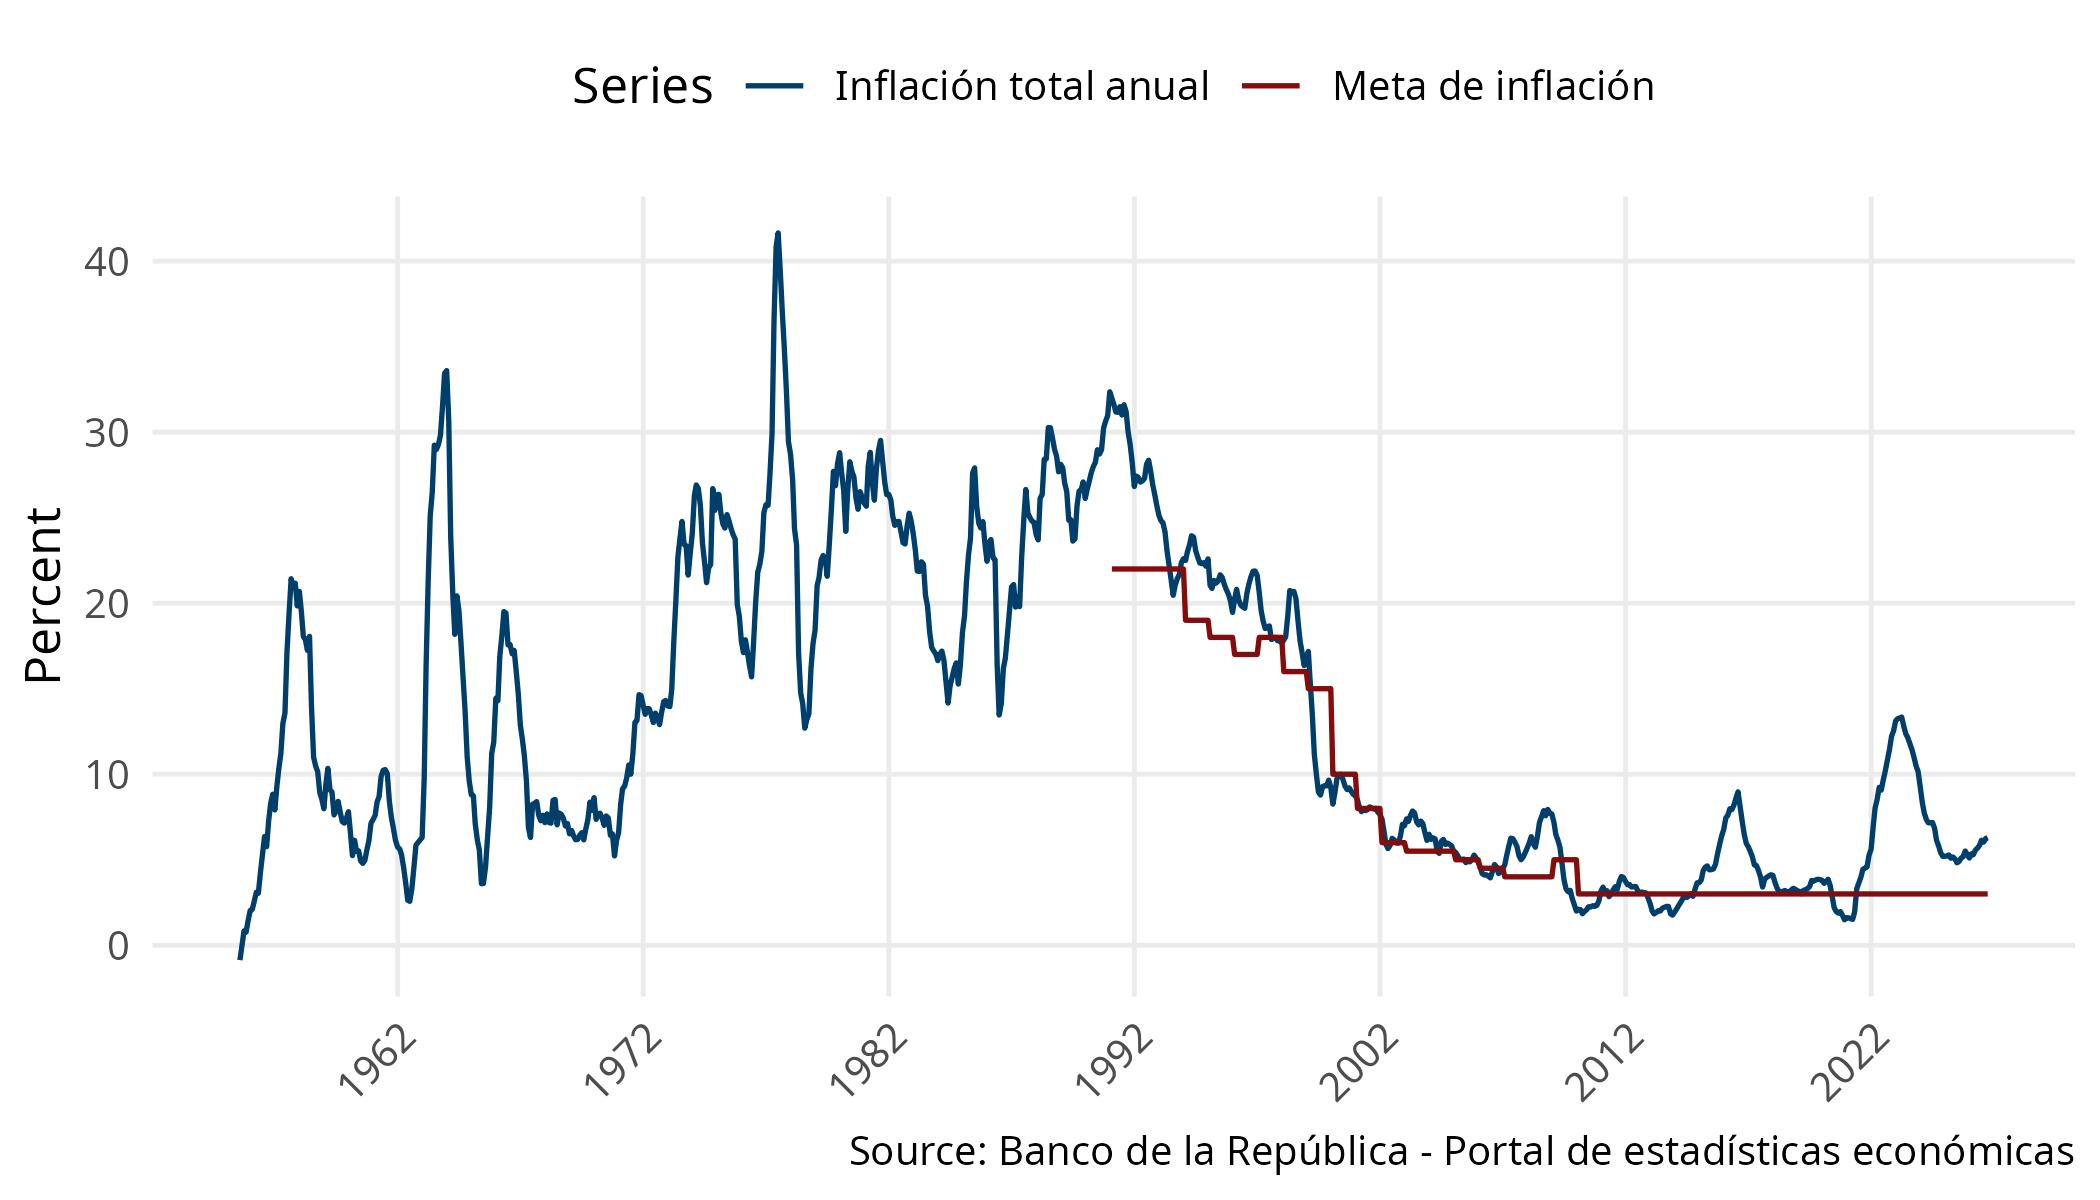
\includegraphics[width=0.48\textwidth]{
banrepstats-precios.png}}
\caption{Output of Listing~\ref{lst:plot}: Colombia's inflation target and realized annual inflation.}
\label{fig:precios}
\end{figure}

\subsection{Forecasting Integration}
Listing~\ref{lst:example} retrieves Colombia's national unemployment rate
(308 monthly observations, January 2001 to August 2026) and fits four
forecasting models from the tidyverts ecosystem
\cite{b_fable, b_hyndman, b_prophet}, including \texttt{NNETAR()}, a
feed-forward neural network autoregression model, on top of the tidy
output of \texttt{banrep\_data()}, requiring only a single conversion
step (\texttt{as\_tsibble()}) to bridge the two ecosystems.

\begin{lstlisting}[caption={Downloading and forecasting an indicator},label={lst:example}]
library(banrepstats); library(fable)
d <- banrep_data(
  "mercado_laboral_poblacion_tasa_ocupacion_desempleo"
) |>
  dplyr::filter(id == "Tasa de desempleo - total nacional") |>
  dplyr::mutate(mes = tsibble::yearmonth(date)) |>
  tsibble::as_tsibble(index = mes)

fit <- d |> model(
  arima  = ARIMA(value),
  ets    = ETS(value),
  nnetar = NNETAR(value),
  prophet = fable.prophet::prophet(value ~
    season(period = 12, order = 5,
           type = "multiplicative"))
)
fit |> forecast(h = "18 months") |> autoplot(d)
\end{lstlisting}

\begin{figure}[htbp]
\centerline{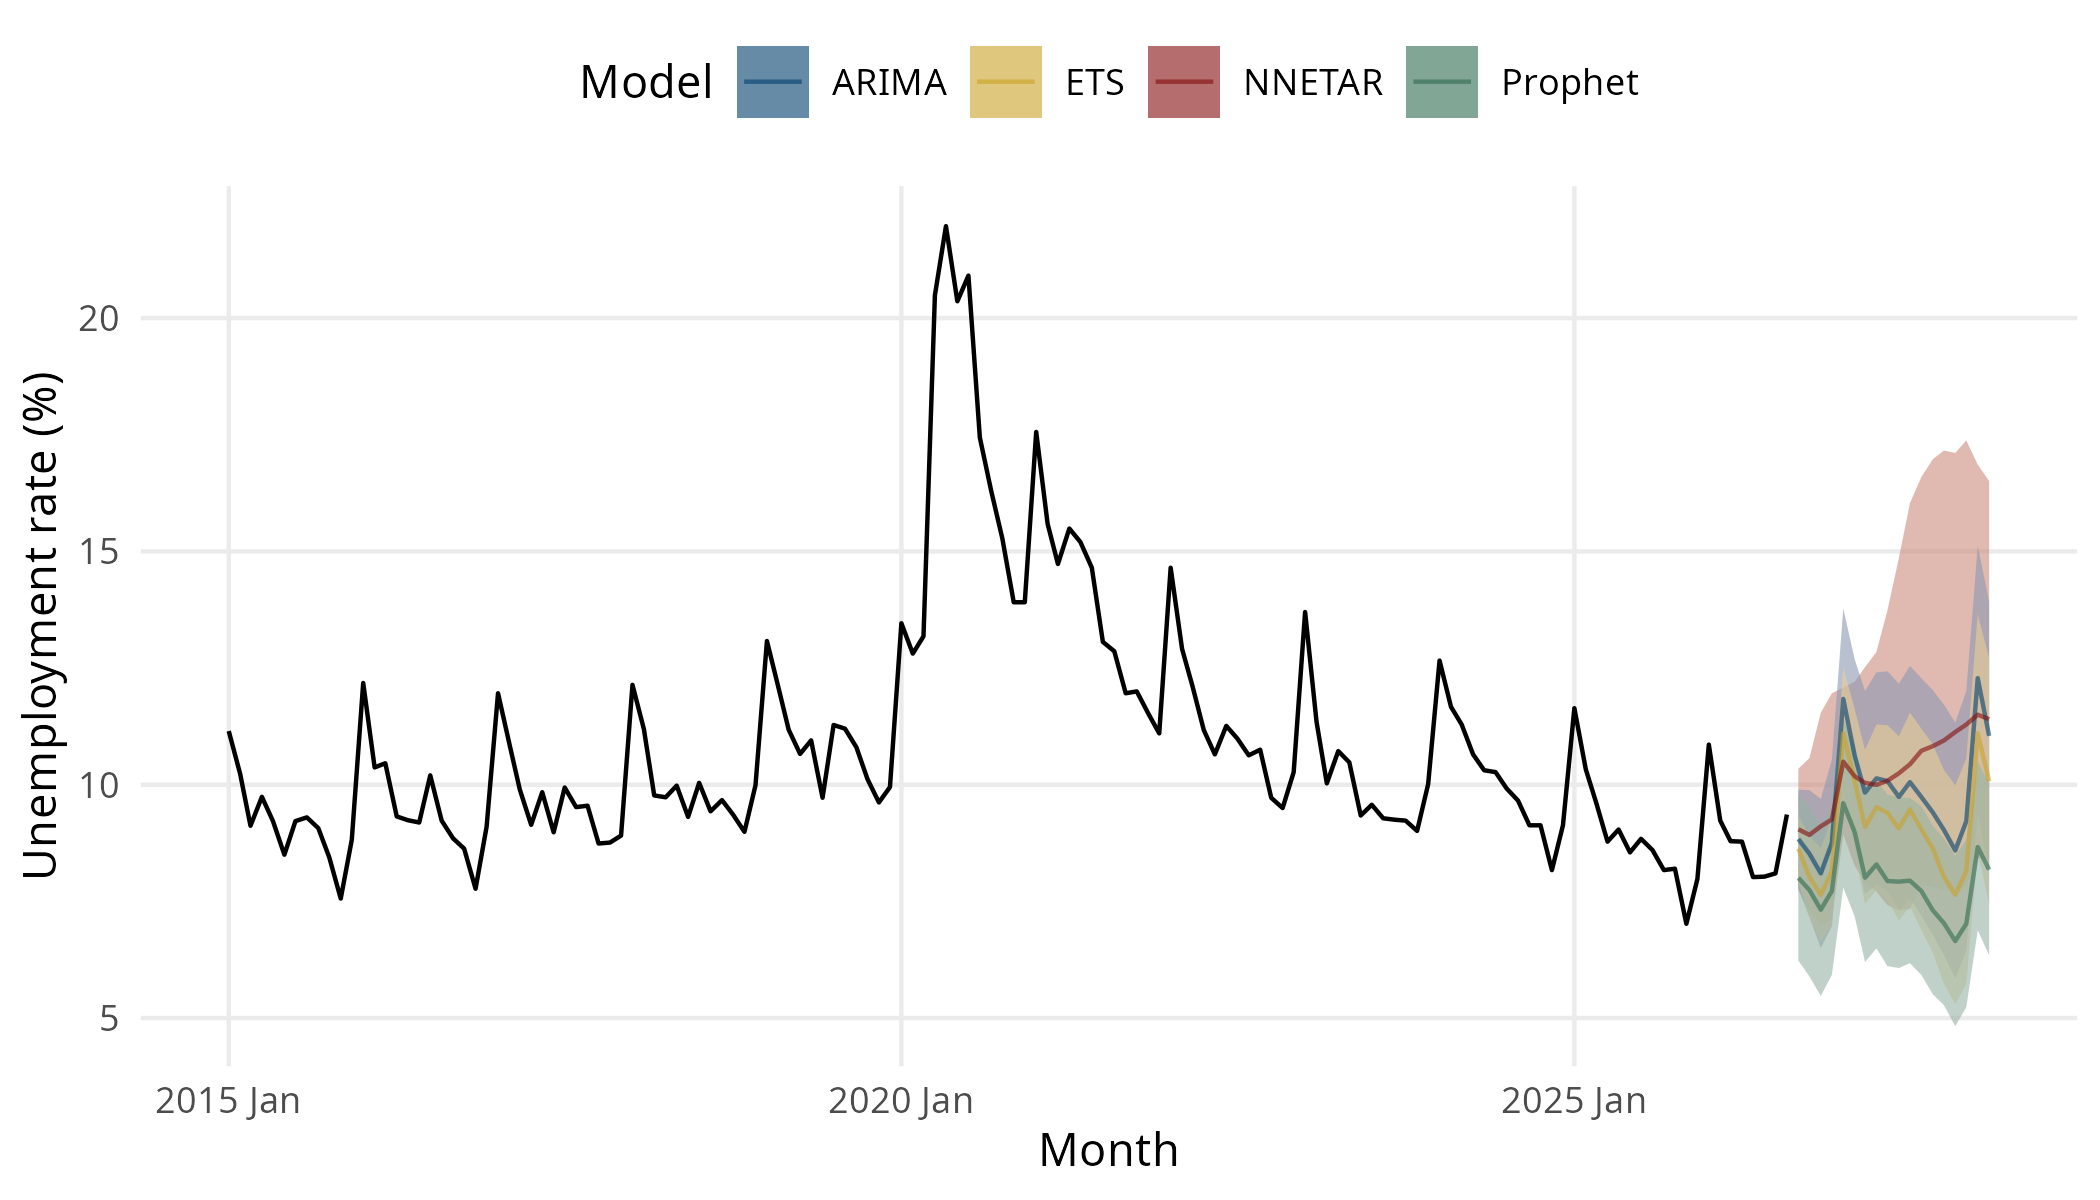
\includegraphics[width=0.48\textwidth]{banrepstats-forecast.png}}
\caption{18-month forecast of Colombia's national unemployment rate, produced from data retrieved with \texttt{banrep\_data()}. Models fitted on the full sample; shaded areas are 80\% prediction intervals; history shown from 2015.}
\label{fig:forecast}
\end{figure}

Fig.~\ref{fig:forecast} shows the resulting 18-month forecast. Producing
this plot requires no manual data wrangling beyond the single
\texttt{tsibble} conversion, illustrating the package's goal: making
Banrep data a first-class citizen of standard R analysis pipelines.

\subsection{A Second Case: Quarterly GDP Growth}
To confirm that the same workflow generalizes across frequencies, we
repeat the exercise on Colombia's quarterly year-on-year real GDP growth
rate (2006Q1--2026Q2, 82 observations), whose code is found with
\texttt{search\_banrep("PIB")}. Only
the conversion step and the seasonal settings change: the index is built
with \texttt{yearquarter()} instead of \texttt{yearmonth()}, and
Prophet uses an additive seasonality of period four and order two
instead of a multiplicative one of period twelve and order five. In both
examples the seasonal period is matched to the frequency of the data.
Fig.~\ref{fig:pib} shows the resulting two-year forecast.


\begin{figure}[htbp]
\centerline{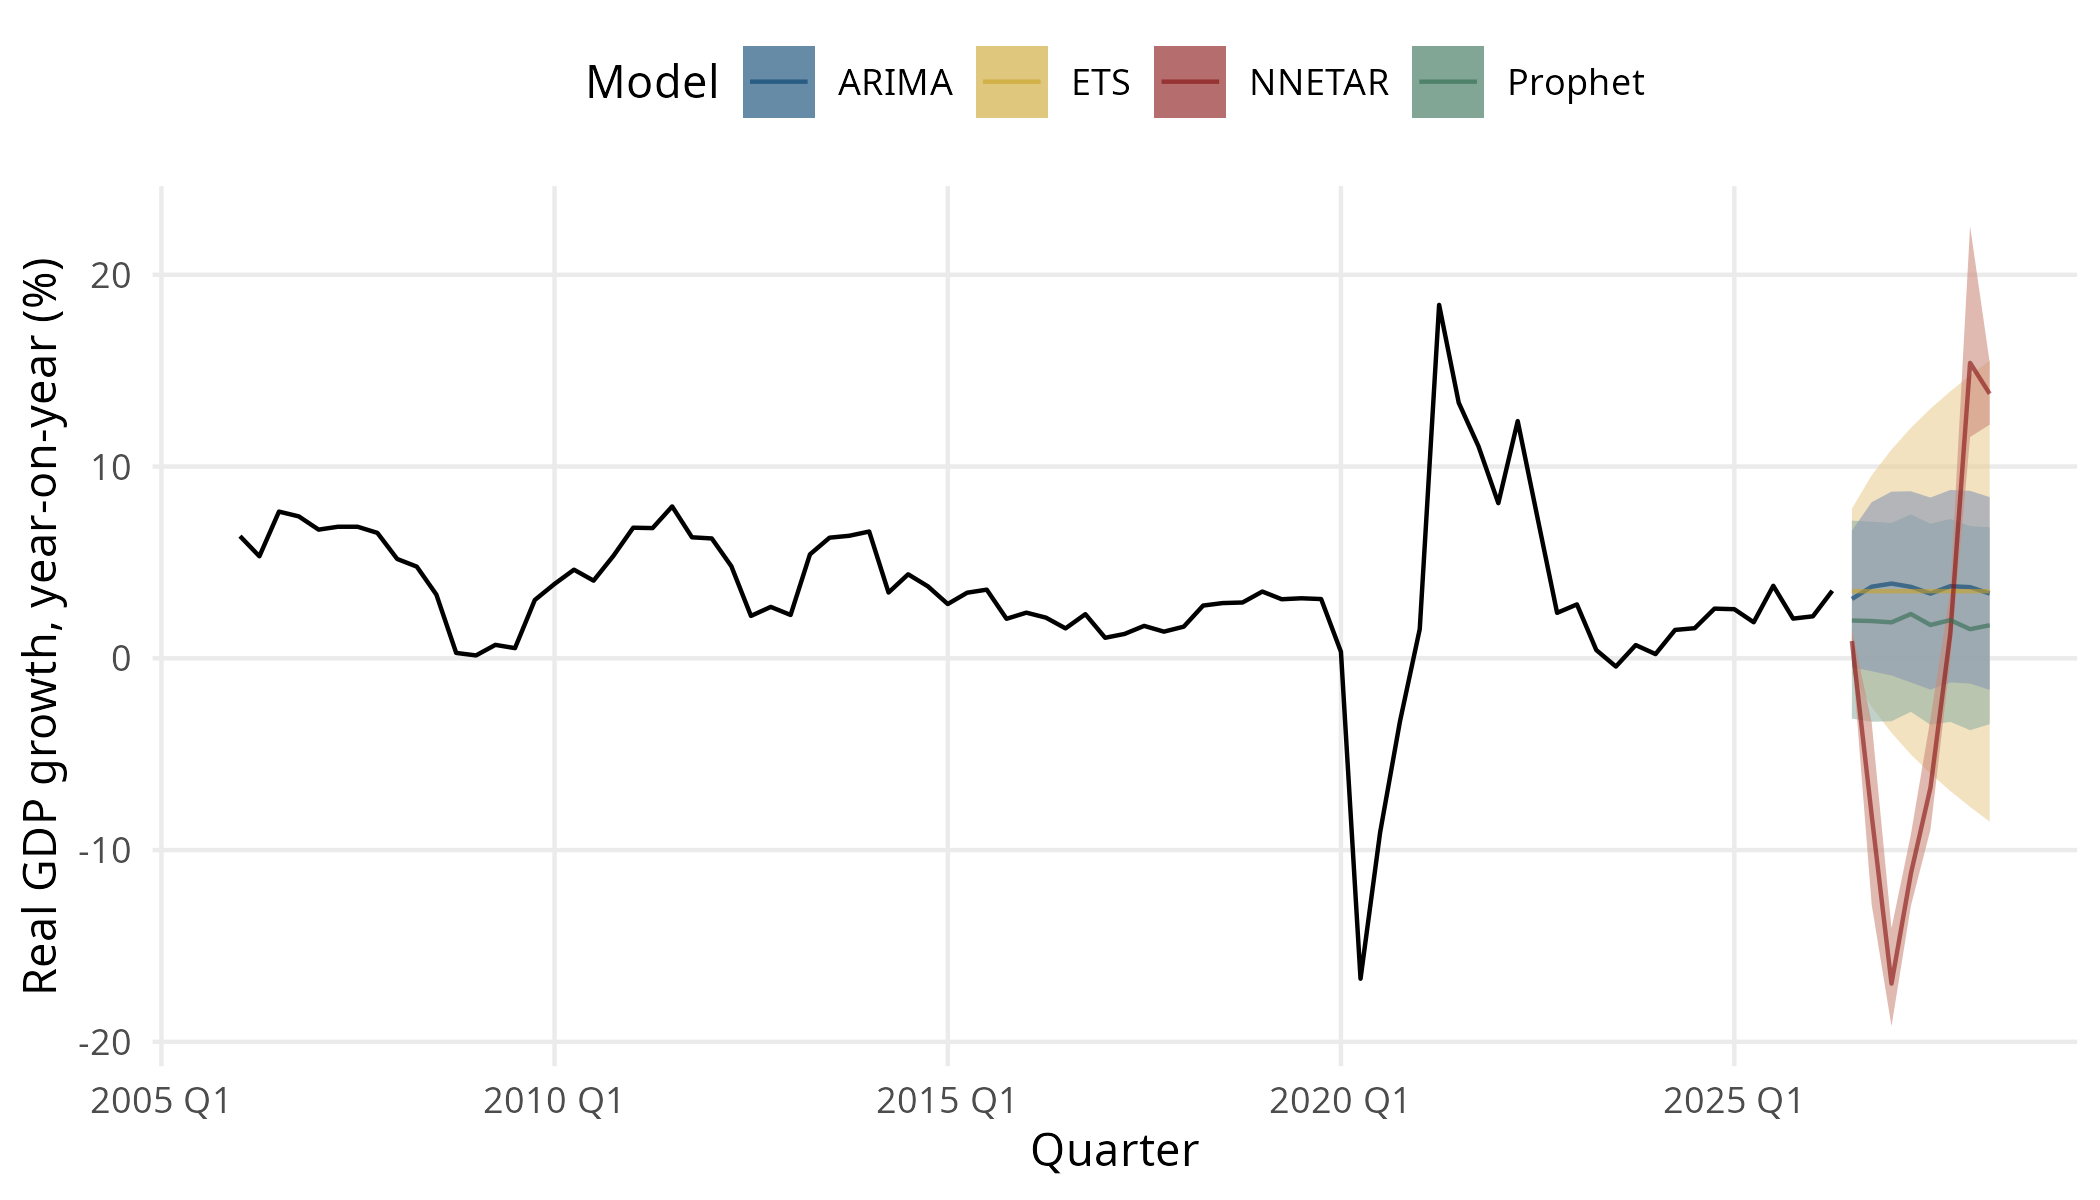
\includegraphics[width=0.48\textwidth]{banrepstats-pib.png}}
\caption{Two-year forecast of Colombia's quarterly year-on-year GDP growth. Models fitted on the full sample; shaded areas are 80\% prediction intervals.}
\label{fig:pib}
\end{figure}

\section{Forecast Accuracy Evaluation}

The purpose of this section is to show that the output of
\texttt{banrep\_data()} supports a complete forecasting workflow,
including out-of-sample evaluation, rather than to establish which model
is best: rankings depend on the indicator, the sample and the evaluation
window, and a single holdout per series is not a basis for general
conclusions about the models.

We hold out the last 10 quarters of GDP growth (2024Q1--2026Q2; 72
training observations, 2006Q1--2023Q4) and the last 10 months of the
unemployment rate (November 2025 to August 2026; 298 training
observations, January 2001 to October 2025), refit each model on the
training data, and score the forecasts against the held-out observations
with \texttt{fabletools::accuracy()}. Table~\ref{tab:accuracy} reports
the root-mean-squared error (RMSE), the mean absolute error (MAE), the
mean absolute percentage error (MAPE) and the mean absolute scaled error
(MASE) \cite{b_hyndman}.

\begin{table}[htbp]
\caption{Out-of-sample forecast accuracy by model and indicator}
\begin{center}
\begin{tabular}{llrrrr}
\toprule
\textbf{Indicator} & \textbf{Model} & \textbf{RMSE} & \textbf{MAE} & \textbf{MAPE} & \textbf{MASE} \\
\midrule
Unemployment & ARIMA    & 0.56 & 0.49 &   5.7 & 0.39 \\
Unemployment & ETS      & 1.06 & 0.96 &  11.5 & 0.77 \\
Unemployment & NNETAR   & 1.23 & 1.12 &  13.6 & 0.89 \\
Unemployment & Prophet  & 0.81 & 0.73 &   8.9 & 0.58 \\
\addlinespace
GDP growth   & ARIMA    & 2.07 & 1.78 & 149.2 & 0.43 \\
GDP growth   & ETS      & 1.79 & 1.60 &  83.0 & 0.39 \\
GDP growth   & NNETAR   & 4.60 & 4.26 & 334.7 & 1.04 \\
GDP growth   & Prophet  & 1.02 & 0.80 & 115.3 & 0.20 \\
\bottomrule
\multicolumn{6}{l}{RMSE and MAE in percentage points; MAPE in \%.}
\end{tabular}
\label{tab:accuracy}
\end{center}
\end{table}

For the unemployment rate, ARIMA attains the lowest error on all four
metrics, consistent with a smooth, strongly autocorrelated monthly
series; Prophet ranks second, followed by ETS, with \texttt{NNETAR()}
last. For GDP growth the ranking changes: Prophet attains the lowest
RMSE, MAE and MASE, followed by ETS and ARIMA, and \texttt{NNETAR()}
performs worst of all four models. MAPE is unreliable for this
indicator, because realized growth in the test window comes as close to
zero as 0.22 percentage points, inflating every model's percentage
error; this is why we also report MASE, which scales errors by the
in-sample error of a seasonal naive forecast and stays well defined near
zero, and ranks the GDP models in the same order as RMSE and MAE.

A plausible explanation for the poor GDP result of \texttt{NNETAR()} is
overfitting. The automatically selected specification,
NNAR(9,1,5)$_4$, has nine lagged inputs and five hidden units, i.e.\ 56
weights per network, estimated from only 63 training patterns, and its
training sample contains the 2020 pandemic collapse and rebound. Two
observations are consistent with this explanation: its in-sample RMSE
(0.37) is twelve times smaller than its out-of-sample RMSE (4.60),
whereas the other three models have out-of-sample errors below their
in-sample errors; and its forecast in Fig.~\ref{fig:pib} reproduces a
pandemic-like collapse and rebound that no other model predicts. For
unemployment, where \texttt{NNETAR()} selects a much smaller
NNAR(1,1,2)$_{12}$ network with nearly 300 training observations, the
gap between in-sample and out-of-sample error is small. These results do
not prove overfitting, but they make it the most likely explanation.

\emph{Reproducibility.} The data were retrieved on October 24, 2026, and
are frozen in the replication materials, since Banrep revises and
extends its series. The results were produced with R 4.5.2,
banrepstats 0.1.1 (whose code is unchanged in version 1.1.0),
\texttt{fable} 0.5.0, \texttt{fabletools} 0.8.0,
\texttt{fable.prophet} 0.1.0 and \texttt{tsibble} 1.2.0, with the random
seed 20261024 reset before each set of models. The script
\texttt{paper/forecast\_eval.R} regenerates Table~\ref{tab:accuracy} and
Figs.~\ref{fig:precios}--\ref{fig:pib}.

\section{Discussion and Limitations}

banrepstats depends on an internal API that Banrep does not commit to
maintaining, so future changes to the SUAMECA application could break the
package without notice. We mitigate this risk at four levels. First, the
package detects changes instead of hiding them: responses are checked
against the fields it relies on, and empty or malformed responses stop
with an explicit error. Second, the offline test suite pins down the
expected format of each response, while the live tests check that the
real service still matches it. Third, the weekly monitoring job of the
package repository runs those live tests, so a breaking change is noticed within
days and fixed in a new release; the blank-slug change described in
Section~IV-C is an example of the kind of change this is meant to catch.
Fourth, the bundled \texttt{banrep\_cache} dataset gives callers an
offline fallback for catalog lookups. None of these measures can prevent
a breaking change, and a documented, versioned public API from Banrep
would remain the most robust solution.
The endpoint also returns each indicator's full history with no
server-side date filtering; the \texttt{start} and \texttt{end}
arguments of \texttt{banrep\_data()} filter after the download, which is
convenient but does not reduce the amount of data transferred. Field and
category names throughout the catalog are in Spanish, which is faithful
to the source but may require translation layers for
non-Spanish-speaking users.

\section{Conclusion}

We presented banrepstats, an R package that turns Banco de la
Rep\'ublica's internal statistics API into a small, tidy, and
forecasting-ready interface for R users. Beyond the package itself, we
documented four concrete failure modes of consuming an undocumented
government API -- silent header-based filtering, timezone-dependent
timestamp drift, unstable or non-unique identifiers, and an incomplete
TLS certificate chain -- that we expect recur when wrapping similar
open-data sources elsewhere in the region. We showed that the package
retrieves the full catalog and reproduces the portal's official exports
exactly. Future work includes CRAN distribution, English-language aliases
for catalog fields, and working with Banrep toward a documented public
API.

\section*{Acknowledgment}
The authors thank the maintainers of the open-source R packages this
project builds on, in particular \texttt{data.table}, \texttt{httr2}, and
the tidyverts forecasting ecosystem.

\begin{thebibliography}{00}
\bibitem{b_rsdmx} E. Blondel, ``rsdmx: Tools for Reading SDMX Data and Metadata,'' R package version 0.6-5, Comprehensive R Archive Network (CRAN), 2025.
\bibitem{b_rbcb} W. Freitas, ``rbcb: R Interface to Brazilian Central Bank Web Services,'' R package version 0.1.14, Comprehensive R Archive Network (CRAN), 2024.
\bibitem{b_wbstats} M. Vargas Sepulveda, ``wbstats: Programmatic Access to the World Bank API,'' Oak Ridge National Laboratory, Oak Ridge, TN, 2025. [Online]. Available: https://doi.org/10.11578/dc.20171025.1827
\bibitem{b_eurostat} L. Lahti, J. Huovari, M. Kainu, and P. Biecek, ``Retrieval and analysis of Eurostat open data with the eurostat package,'' \emph{The R Journal}, vol. 9, no. 1, pp. 385--392, 2017.
\bibitem{b_datatable} T. Barrett, M. Dowle, A. Srinivasan, J. Gorecki, M. Chirico, T. Hocking, B. Schwendinger, and I. Krylov, ``data.table: Extension of `data.frame`,'' R package version 1.18.6.1, Comprehensive R Archive Network (CRAN), 2026.
\bibitem{b_fable} M. O'Hara-Wild, R. Hyndman, and E. Wang, ``fable: Forecasting Models for Tidy Time Series,'' R package version 0.5.0, Comprehensive R Archive Network (CRAN), 2026.
\bibitem{b_hyndman} R. J. Hyndman and G. Athanasopoulos, \emph{Forecasting: Principles and Practice}, 3rd ed. Melbourne: OTexts, 2021.
\bibitem{b_prophet} S. J. Taylor and B. Letham, ``Forecasting at scale,'' \emph{The American Statistician}, vol. 72, no. 1, pp. 37--45, 2018.
\bibitem{b_wickham} H. Wickham, \emph{ggplot2: Elegant Graphics for Data Analysis}, 2nd ed. New York: Springer-Verlag, 2016.
\bibitem{b_httr2} H. Wickham, ``httr2: Perform HTTP Requests and Process the Responses,'' R package version 1.3.0, Comprehensive R Archive Network (CRAN), 2026.
\bibitem{b_testthat} H. Wickham, ``testthat: Get Started with Testing,'' \emph{The R Journal}, vol. 3, no. 1, pp. 5--10, 2011.
\bibitem{b_covr} J. Hester, ``covr: Test Coverage for Packages,'' R package version 3.6.5, Comprehensive R Archive Network (CRAN), 2025.
\end{thebibliography}

\end{document}
